\documentclass[]{article}
\usepackage{lmodern}
\usepackage{amssymb,amsmath}
\usepackage{ifxetex,ifluatex}
\usepackage{fixltx2e} % provides \textsubscript
\ifnum 0\ifxetex 1\fi\ifluatex 1\fi=0 % if pdftex
  \usepackage[T1]{fontenc}
  \usepackage[utf8]{inputenc}
\else % if luatex or xelatex
  \ifxetex
    \usepackage{mathspec}
  \else
    \usepackage{fontspec}
  \fi
  \defaultfontfeatures{Ligatures=TeX,Scale=MatchLowercase}
\fi
% use upquote if available, for straight quotes in verbatim environments
\IfFileExists{upquote.sty}{\usepackage{upquote}}{}
% use microtype if available
\IfFileExists{microtype.sty}{%
\usepackage{microtype}
\UseMicrotypeSet[protrusion]{basicmath} % disable protrusion for tt fonts
}{}
\usepackage[margin=1in]{geometry}
\usepackage{hyperref}
\hypersetup{unicode=true,
            pdftitle={Alfredo Rojas - BIS Data Analyst - Visualization Demo},
            pdfborder={0 0 0},
            breaklinks=true}
\urlstyle{same}  % don't use monospace font for urls
\usepackage{color}
\usepackage{fancyvrb}
\newcommand{\VerbBar}{|}
\newcommand{\VERB}{\Verb[commandchars=\\\{\}]}
\DefineVerbatimEnvironment{Highlighting}{Verbatim}{commandchars=\\\{\}}
% Add ',fontsize=\small' for more characters per line
\usepackage{framed}
\definecolor{shadecolor}{RGB}{248,248,248}
\newenvironment{Shaded}{\begin{snugshade}}{\end{snugshade}}
\newcommand{\AlertTok}[1]{\textcolor[rgb]{0.94,0.16,0.16}{#1}}
\newcommand{\AnnotationTok}[1]{\textcolor[rgb]{0.56,0.35,0.01}{\textbf{\textit{#1}}}}
\newcommand{\AttributeTok}[1]{\textcolor[rgb]{0.77,0.63,0.00}{#1}}
\newcommand{\BaseNTok}[1]{\textcolor[rgb]{0.00,0.00,0.81}{#1}}
\newcommand{\BuiltInTok}[1]{#1}
\newcommand{\CharTok}[1]{\textcolor[rgb]{0.31,0.60,0.02}{#1}}
\newcommand{\CommentTok}[1]{\textcolor[rgb]{0.56,0.35,0.01}{\textit{#1}}}
\newcommand{\CommentVarTok}[1]{\textcolor[rgb]{0.56,0.35,0.01}{\textbf{\textit{#1}}}}
\newcommand{\ConstantTok}[1]{\textcolor[rgb]{0.00,0.00,0.00}{#1}}
\newcommand{\ControlFlowTok}[1]{\textcolor[rgb]{0.13,0.29,0.53}{\textbf{#1}}}
\newcommand{\DataTypeTok}[1]{\textcolor[rgb]{0.13,0.29,0.53}{#1}}
\newcommand{\DecValTok}[1]{\textcolor[rgb]{0.00,0.00,0.81}{#1}}
\newcommand{\DocumentationTok}[1]{\textcolor[rgb]{0.56,0.35,0.01}{\textbf{\textit{#1}}}}
\newcommand{\ErrorTok}[1]{\textcolor[rgb]{0.64,0.00,0.00}{\textbf{#1}}}
\newcommand{\ExtensionTok}[1]{#1}
\newcommand{\FloatTok}[1]{\textcolor[rgb]{0.00,0.00,0.81}{#1}}
\newcommand{\FunctionTok}[1]{\textcolor[rgb]{0.00,0.00,0.00}{#1}}
\newcommand{\ImportTok}[1]{#1}
\newcommand{\InformationTok}[1]{\textcolor[rgb]{0.56,0.35,0.01}{\textbf{\textit{#1}}}}
\newcommand{\KeywordTok}[1]{\textcolor[rgb]{0.13,0.29,0.53}{\textbf{#1}}}
\newcommand{\NormalTok}[1]{#1}
\newcommand{\OperatorTok}[1]{\textcolor[rgb]{0.81,0.36,0.00}{\textbf{#1}}}
\newcommand{\OtherTok}[1]{\textcolor[rgb]{0.56,0.35,0.01}{#1}}
\newcommand{\PreprocessorTok}[1]{\textcolor[rgb]{0.56,0.35,0.01}{\textit{#1}}}
\newcommand{\RegionMarkerTok}[1]{#1}
\newcommand{\SpecialCharTok}[1]{\textcolor[rgb]{0.00,0.00,0.00}{#1}}
\newcommand{\SpecialStringTok}[1]{\textcolor[rgb]{0.31,0.60,0.02}{#1}}
\newcommand{\StringTok}[1]{\textcolor[rgb]{0.31,0.60,0.02}{#1}}
\newcommand{\VariableTok}[1]{\textcolor[rgb]{0.00,0.00,0.00}{#1}}
\newcommand{\VerbatimStringTok}[1]{\textcolor[rgb]{0.31,0.60,0.02}{#1}}
\newcommand{\WarningTok}[1]{\textcolor[rgb]{0.56,0.35,0.01}{\textbf{\textit{#1}}}}
\usepackage{graphicx,grffile}
\makeatletter
\def\maxwidth{\ifdim\Gin@nat@width>\linewidth\linewidth\else\Gin@nat@width\fi}
\def\maxheight{\ifdim\Gin@nat@height>\textheight\textheight\else\Gin@nat@height\fi}
\makeatother
% Scale images if necessary, so that they will not overflow the page
% margins by default, and it is still possible to overwrite the defaults
% using explicit options in \includegraphics[width, height, ...]{}
\setkeys{Gin}{width=\maxwidth,height=\maxheight,keepaspectratio}
\IfFileExists{parskip.sty}{%
\usepackage{parskip}
}{% else
\setlength{\parindent}{0pt}
\setlength{\parskip}{6pt plus 2pt minus 1pt}
}
\setlength{\emergencystretch}{3em}  % prevent overfull lines
\providecommand{\tightlist}{%
  \setlength{\itemsep}{0pt}\setlength{\parskip}{0pt}}
\setcounter{secnumdepth}{0}
% Redefines (sub)paragraphs to behave more like sections
\ifx\paragraph\undefined\else
\let\oldparagraph\paragraph
\renewcommand{\paragraph}[1]{\oldparagraph{#1}\mbox{}}
\fi
\ifx\subparagraph\undefined\else
\let\oldsubparagraph\subparagraph
\renewcommand{\subparagraph}[1]{\oldsubparagraph{#1}\mbox{}}
\fi

%%% Use protect on footnotes to avoid problems with footnotes in titles
\let\rmarkdownfootnote\footnote%
\def\footnote{\protect\rmarkdownfootnote}

%%% Change title format to be more compact
\usepackage{titling}

% Create subtitle command for use in maketitle
\providecommand{\subtitle}[1]{
  \posttitle{
    \begin{center}\large#1\end{center}
    }
}

\setlength{\droptitle}{-2em}

  \title{Alfredo Rojas - BIS Data Analyst - Visualization Demo}
    \pretitle{\vspace{\droptitle}\centering\huge}
  \posttitle{\par}
    \author{}
    \preauthor{}\postauthor{}
    \date{}
    \predate{}\postdate{}
  
\usepackage{graphicx}

\begin{document}
\maketitle

\hypertarget{visualization-demo}{%
\section{Visualization demo}\label{visualization-demo}}

\hypertarget{started-by-importing-libraries}{%
\subsection{Started by importing
libraries}\label{started-by-importing-libraries}}

\begin{Shaded}
\begin{Highlighting}[]
\KeywordTok{library}\NormalTok{(dplyr)}
\KeywordTok{library}\NormalTok{(tidyr)}
\KeywordTok{library}\NormalTok{(ggplot2)}
\KeywordTok{library}\NormalTok{(plotly)}
\KeywordTok{library}\NormalTok{(stringr)}
\KeywordTok{library}\NormalTok{(DataExplorer)}
\end{Highlighting}
\end{Shaded}

\hypertarget{and-loading-the-dataset}{%
\subsection{And loading the dataset}\label{and-loading-the-dataset}}

\begin{Shaded}
\begin{Highlighting}[]
\KeywordTok{setwd}\NormalTok{(}\StringTok{"C:/Users/alfrs/Documents/git/RProjects/Experian"}\NormalTok{)}
\NormalTok{dataset <-}\StringTok{ }\NormalTok{readxl}\OperatorTok{::}\KeywordTok{read_xlsx}\NormalTok{(}\StringTok{"DATA_FILE_FOR_INTERVIEW.xlsx"}\NormalTok{)}
\KeywordTok{head}\NormalTok{(dataset)}
\end{Highlighting}
\end{Shaded}

\begin{verbatim}
## # A tibble: 6 x 10
##   COMPANY_NAME CITY  STATE ZIP   COUNTRY PHONE YEAR_INCORP ANNUAL_SALES
##   <chr>        <chr> <chr> <chr> <chr>   <chr> <chr>              <dbl>
## 1 AAR Corp     Wood~ IL    60191 USA     630 ~ 1955          2051800000
## 2 AFA Protect~ Syos~ NY    11791 USA     516 ~ 1873            73220115
## 3 American Lo~ DFW ~ TX    75261 USA     817 ~ 1898            14625889
## 4 Abbott Labo~ Abbo~ IL    60064 USA     224 ~ 1900         30578000000
## 5 ACMAT Corp.  Farm~ CT    06032 USA     860 ~ 1951             2750729
## 6 Acme United~ Fair~ CT    06824 USA     203 ~ 1867           137321395
## # ... with 2 more variables: EMPLOYEE_COUNT <dbl>, NET_INCOME <dbl>
\end{verbatim}

\hypertarget{then-i-checked-column-types-and-reassigned-those-i-thought-needed-reassignment}{%
\subsection{Then I checked column types and reassigned those I thought
needed
reassignment}\label{then-i-checked-column-types-and-reassigned-those-i-thought-needed-reassignment}}

\begin{Shaded}
\begin{Highlighting}[]
\KeywordTok{str}\NormalTok{(dataset)}
\end{Highlighting}
\end{Shaded}

\begin{verbatim}
## Classes 'tbl_df', 'tbl' and 'data.frame':    8382 obs. of  10 variables:
##  $ COMPANY_NAME  : chr  "AAR Corp" "AFA Protective Systems, Inc." "American Locker Group, Inc." "Abbott Laboratories" ...
##  $ CITY          : chr  "Wood Dale" "Syosset" "DFW Airport" "Abbott Park" ...
##  $ STATE         : chr  "IL" "NY" "TX" "IL" ...
##  $ ZIP           : chr  "60191" "11791" "75261" "60064" ...
##  $ COUNTRY       : chr  "USA" "USA" "USA" "USA" ...
##  $ PHONE         : chr  "630 227-2000" "516 496-2322" "817 329-1600" "224 667-6100" ...
##  $ YEAR_INCORP   : chr  "1955" "1873" "1898" "1900" ...
##  $ ANNUAL_SALES  : num  2.05e+09 7.32e+07 1.46e+07 3.06e+10 2.75e+06 ...
##  $ EMPLOYEE_COUNT: num  6550 0 120 103000 NA 435 703 10100 16300 570 ...
##  $ NET_INCOME    : num  7.50e+06 2.60e+05 -2.82e+06 2.37e+09 7.44e+05 ...
\end{verbatim}

\begin{Shaded}
\begin{Highlighting}[]
\NormalTok{dataset}\OperatorTok{$}\NormalTok{COMPANY_NAME <-}\StringTok{ }\KeywordTok{as.factor}\NormalTok{(dataset}\OperatorTok{$}\NormalTok{COMPANY_NAME)}
\NormalTok{dataset}\OperatorTok{$}\NormalTok{CITY <-}\StringTok{ }\KeywordTok{as.factor}\NormalTok{(dataset}\OperatorTok{$}\NormalTok{CITY)}
\NormalTok{dataset}\OperatorTok{$}\NormalTok{STATE <-}\StringTok{ }\KeywordTok{as.factor}\NormalTok{(dataset}\OperatorTok{$}\NormalTok{STATE)}
\NormalTok{dataset}\OperatorTok{$}\NormalTok{ZIP <-}\StringTok{ }\KeywordTok{as.factor}\NormalTok{(dataset}\OperatorTok{$}\NormalTok{ZIP)}
\NormalTok{dataset}\OperatorTok{$}\NormalTok{COUNTRY <-}\StringTok{ }\KeywordTok{as.factor}\NormalTok{(dataset}\OperatorTok{$}\NormalTok{COUNTRY)}
\NormalTok{dataset}\OperatorTok{$}\NormalTok{PHONE <-}\StringTok{ }\KeywordTok{as.factor}\NormalTok{(dataset}\OperatorTok{$}\NormalTok{PHONE)}
\NormalTok{dataset}\OperatorTok{$}\NormalTok{YEAR_INCORP <-}\StringTok{ }\KeywordTok{as.numeric}\NormalTok{(dataset}\OperatorTok{$}\NormalTok{YEAR_INCORP)}
\NormalTok{dataset}\OperatorTok{$}\NormalTok{ANNUAL_SALES <-}\StringTok{ }\KeywordTok{as.double}\NormalTok{(dataset}\OperatorTok{$}\NormalTok{ANNUAL_SALES)}
\NormalTok{dataset}\OperatorTok{$}\NormalTok{EMPLOYEE_COUNT <-}\StringTok{ }\KeywordTok{as.double}\NormalTok{(dataset}\OperatorTok{$}\NormalTok{EMPLOYEE_COUNT)}
\NormalTok{dataset}\OperatorTok{$}\NormalTok{NET_INCOME <-}\StringTok{ }\KeywordTok{as.double}\NormalTok{(dataset}\OperatorTok{$}\NormalTok{NET_INCOME)}

\KeywordTok{summary}\NormalTok{(dataset)}
\end{Highlighting}
\end{Shaded}

\begin{verbatim}
##                                COMPANY_NAME         CITY     
##  024 Pharma Inc                      :   1   New York : 473  
##  1-800 Flowers.com, Inc.             :   1   Houston  : 262  
##  10x Genomics Inc                    :   1   Las Vegas: 188  
##  11 Good Energy Inc                  :   1   Dallas   : 130  
##  1347 Property Insurance Holdings Inc:   1   San Diego: 109  
##  180 Degree Capital Corp             :   1   (Other)  :7117  
##  (Other)                             :8376   NA's     : 103  
##      STATE           ZIP          COUNTRY              PHONE     
##  CA     :1280   10022  :  84   USA    :7283   800 983-0903:  11  
##  NY     : 739   77002  :  67   CHN    : 308   855 588-7839:   8  
##  TX     : 733   92121  :  47   CAN    : 205   510 522-9600:   7  
##  FL     : 553   80202  :  43   HKG    :  91   512 236-6555:   6  
##  NV     : 315   10019  :  36   ISR    :  80   800 736-3402:   6  
##  (Other):4175   (Other):7968   (Other): 414   (Other)     :8310  
##  NA's   : 587   NA's   : 137   NA's   :   1   NA's        :  34  
##   YEAR_INCORP    ANNUAL_SALES        EMPLOYEE_COUNT   
##  Min.   :1784   Min.   :-2.781e+08   Min.   :      0  
##  1st Qu.:1986   1st Qu.: 4.095e+06   1st Qu.:     13  
##  Median :1999   Median : 8.760e+07   Median :    187  
##  Mean   :1991   Mean   : 2.709e+09   Mean   :   6671  
##  3rd Qu.:2008   3rd Qu.: 9.903e+08   3rd Qu.:   2228  
##  Max.   :2019   Max.   : 5.144e+11   Max.   :2200000  
##  NA's   :157    NA's   :1625         NA's   :1668     
##    NET_INCOME        
##  Min.   :-2.244e+10  
##  1st Qu.:-5.216e+06  
##  Median :-7.610e+04  
##  Mean   : 1.758e+08  
##  3rd Qu.: 2.798e+07  
##  Max.   : 5.953e+10  
##  NA's   :25
\end{verbatim}

\hypertarget{from-this-summary-i-can-see-that}{%
\subsection{From this summary, I can see
that:}\label{from-this-summary-i-can-see-that}}

\hypertarget{a.-we-have-nas-in-year-however-it-does-not-makes-sense-to-change-them-as-year-is-a-very-specific-column.}{%
\subsubsection{A. We have NAs in Year, however, it does not makes sense
to change them as Year is a very specific
column.}\label{a.-we-have-nas-in-year-however-it-does-not-makes-sense-to-change-them-as-year-is-a-very-specific-column.}}

\hypertarget{b.-we-have-nas-in-employee-count.-these-can-be-replaced-well-need-to-analyze-to-determine-with-what.}{%
\subsubsection{B. We have NAs in Employee Count. These can be replaced,
we'll need to analyze to determine with
what.}\label{b.-we-have-nas-in-employee-count.-these-can-be-replaced-well-need-to-analyze-to-determine-with-what.}}

\hypertarget{c.-we-have-nas-in-country.-again-this-is-very-specific-so-we-can-just-exclude-it.}{%
\subsubsection{C. We have NAs in COuntry. Again, this is very specific,
so we can just exclude
it.}\label{c.-we-have-nas-in-country.-again-this-is-very-specific-so-we-can-just-exclude-it.}}

\hypertarget{d.-we-have-nas-in-annual-sales.-this-can-also-be-replaced-so-need-to-analyze-this.}{%
\subsubsection{D. We have NAs in Annual Sales. This can also be
replaced, so need to analyze
this.}\label{d.-we-have-nas-in-annual-sales.-this-can-also-be-replaced-so-need-to-analyze-this.}}

\hypertarget{i-started-working-on-the-first-point.-a-distribution-of-companies-by-year-sounded-very-easy-but-the-graph-said-otherwise.}{%
\subsection{I started working on the first point. A distribution of
companies by year sounded very easy, but the graph said
otherwise.}\label{i-started-working-on-the-first-point.-a-distribution-of-companies-by-year-sounded-very-easy-but-the-graph-said-otherwise.}}

\hypertarget{as-a-matter-of-fact-the-graph-was-so-big-that-it-cant-really-show-in-the-document}{%
\subsection{As a matter of fact, the graph was so big that it can't
really show in the
document}\label{as-a-matter-of-fact-the-graph-was-so-big-that-it-cant-really-show-in-the-document}}

\begin{Shaded}
\begin{Highlighting}[]
\NormalTok{year_graph_}\DecValTok{1}\NormalTok{ <-}\StringTok{ }
\KeywordTok{ggplot}\NormalTok{(dataset }\OperatorTok
\StringTok{         }\KeywordTok{count}\NormalTok{(YEAR_INCORP),}
       \KeywordTok{aes}\NormalTok{(}\DataTypeTok{x =}\NormalTok{ YEAR_INCORP,}
           \DataTypeTok{y =}\NormalTok{ n,}
           \DataTypeTok{fill =} \KeywordTok{as.factor}\NormalTok{(YEAR_INCORP)))}\OperatorTok{+}
\StringTok{  }\KeywordTok{geom_col}\NormalTok{()}\OperatorTok{+}
\StringTok{  }\CommentTok{#geom_text(aes(label = n),position = position_stack(vjust = .5)) +}
\StringTok{  }\KeywordTok{ggtitle}\NormalTok{(}\StringTok{"Count of Companies by Year Bucket"}\NormalTok{)}\OperatorTok{+}
\StringTok{  }\KeywordTok{theme}\NormalTok{(}\DataTypeTok{plot.title =} \KeywordTok{element_text}\NormalTok{(}\DataTypeTok{hjust =} \FloatTok{0.5}\NormalTok{),}
        \DataTypeTok{axis.text.x =} \KeywordTok{element_blank}\NormalTok{(),}
        \DataTypeTok{axis.ticks.x =} \KeywordTok{element_blank}\NormalTok{())}\OperatorTok{+}
\StringTok{  }\KeywordTok{ylab}\NormalTok{(}\StringTok{"Count of Companies by Year"}\NormalTok{) }\OperatorTok{+}
\StringTok{  }\KeywordTok{labs}\NormalTok{(}\DataTypeTok{fill =} \StringTok{"Year Incorporated"}\NormalTok{) }\OperatorTok{+}
\StringTok{  }\KeywordTok{coord_flip}\NormalTok{()}
\end{Highlighting}
\end{Shaded}

\hypertarget{so-then-tried-a-histogram-since-were-using-years-maybe-i-can-see-which-are-the-most-valuable-however}{%
\subsection{So then tried a histogram, since we're using years, maybe I
can see which are the most valuable,
however\ldots{}}\label{so-then-tried-a-histogram-since-were-using-years-maybe-i-can-see-which-are-the-most-valuable-however}}

\begin{Shaded}
\begin{Highlighting}[]
\KeywordTok{ggplot}\NormalTok{(dataset,}\KeywordTok{aes}\NormalTok{(}\DataTypeTok{x =}\NormalTok{ YEAR_INCORP))}\OperatorTok{+}
\StringTok{  }\KeywordTok{geom_histogram}\NormalTok{() }\OperatorTok{+}
\StringTok{  }\KeywordTok{ggtitle}\NormalTok{(}\StringTok{"Number of Companies by Year"}\NormalTok{)}\OperatorTok{+}
\StringTok{  }\KeywordTok{theme}\NormalTok{(}\DataTypeTok{panel.background =} \KeywordTok{element_blank}\NormalTok{(),}
        \DataTypeTok{plot.title =} \KeywordTok{element_text}\NormalTok{(}\DataTypeTok{hjust =} \FloatTok{0.5}\NormalTok{)) }\OperatorTok{+}
\StringTok{  }\KeywordTok{xlab}\NormalTok{(}\StringTok{"Year"}\NormalTok{) }\OperatorTok{+}
\StringTok{  }\KeywordTok{ylab}\NormalTok{(}\StringTok{"Count of Companies"}\NormalTok{)}
\end{Highlighting}
\end{Shaded}

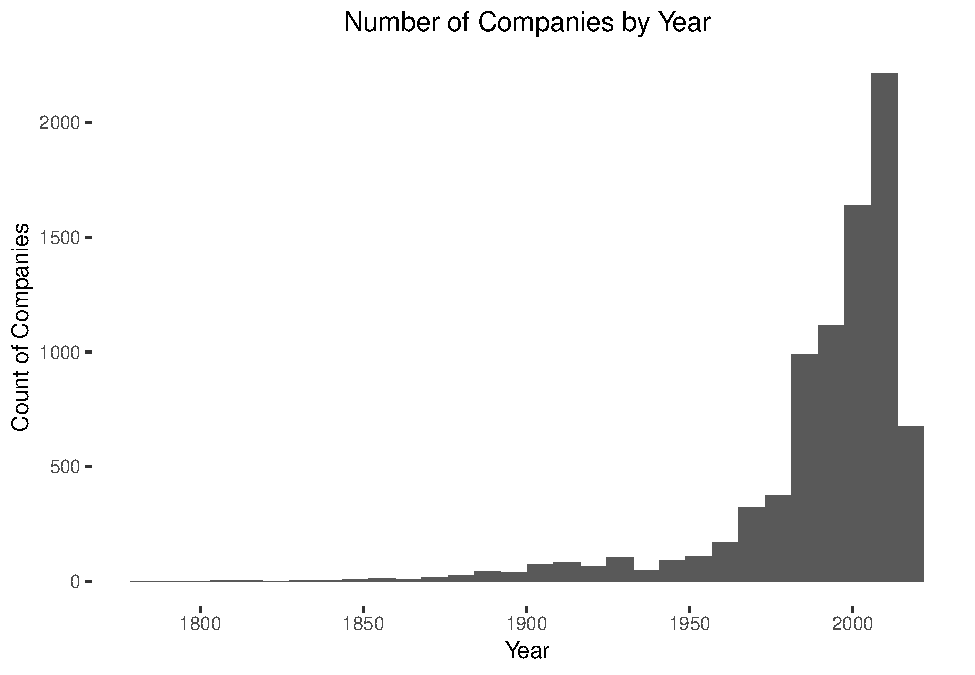
\includegraphics{Main_files/figure-latex/unnamed-chunk-5-1.pdf}

\hypertarget{the-histogram-did-show-me-that-most-of-my-companies-are-arround-the-2000s}{%
\subsection{The histogram did show me that most of my companies are
arround the
2000's}\label{the-histogram-did-show-me-that-most-of-my-companies-are-arround-the-2000s}}

\hypertarget{but-i-cant-really-see-which-year-is-the-most-valuable}{%
\subsection{But I can't really see which year is the most
valuable}\label{but-i-cant-really-see-which-year-is-the-most-valuable}}

\hypertarget{so-i-did-year-buckets-that-would-allow-me-to-graph-and-see-the-data-in-a-more-manageable-way}{%
\subsection{So I did year buckets, that would allow me to graph and see
the data in a more manageable
way}\label{so-i-did-year-buckets-that-would-allow-me-to-graph-and-see-the-data-in-a-more-manageable-way}}

\begin{Shaded}
\begin{Highlighting}[]
\NormalTok{dataset}\OperatorTok{$}\NormalTok{YEAR_BUCKET <-}\StringTok{ }\KeywordTok{cut}\NormalTok{(dataset}\OperatorTok{$}\NormalTok{YEAR_INCORP,}\DataTypeTok{dig.lab=}\DecValTok{4}\NormalTok{,}\DataTypeTok{breaks=}\DecValTok{10}\NormalTok{)}
\NormalTok{dataset}\OperatorTok{$}\NormalTok{YEAR_BUCKET <-}\StringTok{ }\KeywordTok{str_replace}\NormalTok{(dataset}\OperatorTok{$}\NormalTok{YEAR_BUCKET, }\StringTok{"}\CharTok{\textbackslash{}\textbackslash{}}\StringTok{("}\NormalTok{, }\StringTok{""}\NormalTok{)}
\NormalTok{dataset}\OperatorTok{$}\NormalTok{YEAR_BUCKET <-}\StringTok{ }\KeywordTok{str_replace}\NormalTok{(dataset}\OperatorTok{$}\NormalTok{YEAR_BUCKET, }\StringTok{"]"}\NormalTok{, }\StringTok{""}\NormalTok{)}
\NormalTok{dataset}\OperatorTok{$}\NormalTok{YEAR_BUCKET <-}\StringTok{ }\KeywordTok{str_replace}\NormalTok{(dataset}\OperatorTok{$}\NormalTok{YEAR_BUCKET, }\StringTok{","}\NormalTok{, }\StringTok{" - "}\NormalTok{)}

\NormalTok{dataset}\OperatorTok{$}\NormalTok{YEAR_BUCKET <-}\StringTok{ }\KeywordTok{as.factor}\NormalTok{(dataset}\OperatorTok{$}\NormalTok{YEAR_BUCKET)}

\KeywordTok{ggplot}\NormalTok{(}\KeywordTok{na.exclude}\NormalTok{(dataset) }\OperatorTok\StringTok{ }
\StringTok{         }\KeywordTok{count}\NormalTok{(YEAR_BUCKET),}
       \KeywordTok{aes}\NormalTok{(}\DataTypeTok{x =}\NormalTok{ YEAR_BUCKET,}
           \DataTypeTok{y =}\NormalTok{ n,}
           \DataTypeTok{fill =} \KeywordTok{as.factor}\NormalTok{(YEAR_BUCKET)))}\OperatorTok{+}
\StringTok{  }\KeywordTok{geom_col}\NormalTok{()}\OperatorTok{+}
\StringTok{  }\KeywordTok{geom_text}\NormalTok{(}\KeywordTok{aes}\NormalTok{(}\DataTypeTok{label =}\NormalTok{ n),}\DataTypeTok{position =} \KeywordTok{position_stack}\NormalTok{(}\DataTypeTok{vjust =} \FloatTok{.5}\NormalTok{)) }\OperatorTok{+}
\StringTok{  }\KeywordTok{ggtitle}\NormalTok{(}\StringTok{"Count of Companies by Year Bucket"}\NormalTok{)}\OperatorTok{+}
\StringTok{  }\KeywordTok{theme}\NormalTok{(}\DataTypeTok{plot.title =} \KeywordTok{element_text}\NormalTok{(}\DataTypeTok{hjust =} \FloatTok{0.5}\NormalTok{),}
        \DataTypeTok{axis.text.x =} \KeywordTok{element_blank}\NormalTok{(),}
        \DataTypeTok{axis.ticks.x =} \KeywordTok{element_blank}\NormalTok{(),}
        \DataTypeTok{panel.background =} \KeywordTok{element_blank}\NormalTok{())}\OperatorTok{+}
\StringTok{  }\KeywordTok{ylab}\NormalTok{(}\StringTok{"Count of companies"}\NormalTok{) }\OperatorTok{+}
\StringTok{  }\KeywordTok{xlab}\NormalTok{(}\KeywordTok{element_blank}\NormalTok{()) }\OperatorTok{+}
\StringTok{  }\KeywordTok{labs}\NormalTok{(}\DataTypeTok{fill =} \StringTok{"Year Bucket"}\NormalTok{) }\OperatorTok{+}
\StringTok{  }\KeywordTok{coord_flip}\NormalTok{()}
\end{Highlighting}
\end{Shaded}

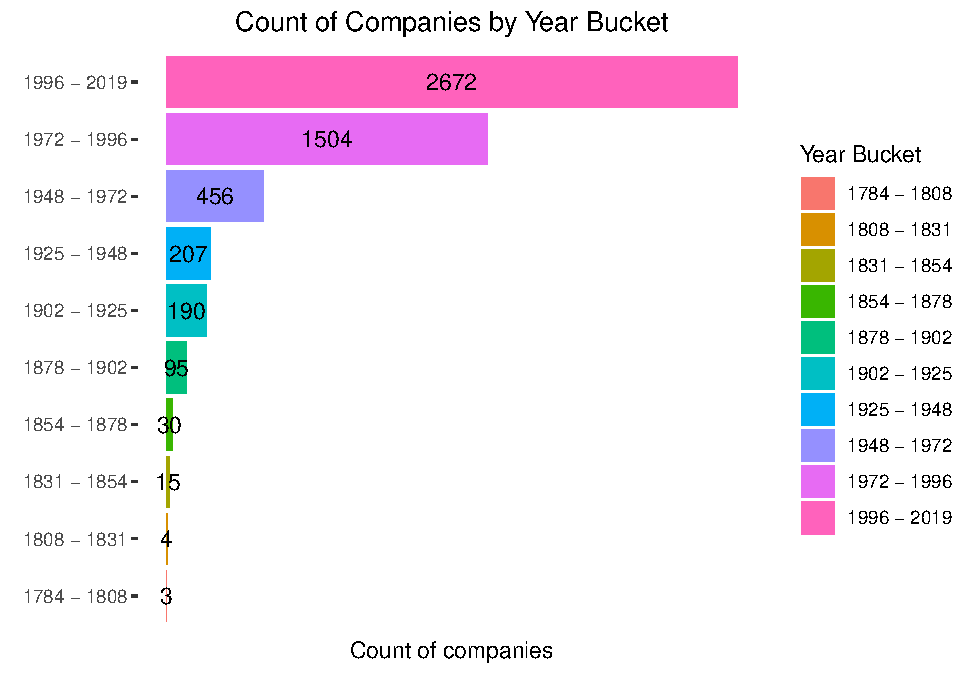
\includegraphics{Main_files/figure-latex/unnamed-chunk-6-1.pdf}

\hypertarget{thanks-to-the-buckets-i-saw-that-most-of-my-data-is-from-1972-going-forward.-so-i-did-buckets-again-but-only-with-these-years.}{%
\subsection{Thanks to the buckets, I saw that most of my data is from
1972 going forward. So I did buckets again, but only with these
years.}\label{thanks-to-the-buckets-i-saw-that-most-of-my-data-is-from-1972-going-forward.-so-i-did-buckets-again-but-only-with-these-years.}}

\begin{Shaded}
\begin{Highlighting}[]
\NormalTok{dataset_filtered <-}\StringTok{ }\NormalTok{dataset }\OperatorTok\StringTok{ }\KeywordTok{filter}\NormalTok{(YEAR_INCORP }\OperatorTok{>=}\StringTok{ }\DecValTok{1972}\NormalTok{)}
\NormalTok{dataset_filtered}\OperatorTok{$}\NormalTok{YEAR_BUCKET <-}\StringTok{ }\KeywordTok{cut}\NormalTok{(dataset_filtered}\OperatorTok{$}\NormalTok{YEAR_INCORP,}\DataTypeTok{dig.lab=}\DecValTok{4}\NormalTok{,}\DataTypeTok{breaks=}\DecValTok{10}\NormalTok{)}
\NormalTok{dataset_filtered}\OperatorTok{$}\NormalTok{YEAR_BUCKET <-}\StringTok{ }\KeywordTok{str_replace}\NormalTok{(dataset_filtered}\OperatorTok{$}\NormalTok{YEAR_BUCKET, }\StringTok{"}\CharTok{\textbackslash{}\textbackslash{}}\StringTok{("}\NormalTok{, }\StringTok{""}\NormalTok{)}
\NormalTok{dataset_filtered}\OperatorTok{$}\NormalTok{YEAR_BUCKET <-}\StringTok{ }\KeywordTok{str_replace}\NormalTok{(dataset_filtered}\OperatorTok{$}\NormalTok{YEAR_BUCKET, }\StringTok{"]"}\NormalTok{, }\StringTok{""}\NormalTok{)}
\NormalTok{dataset_filtered}\OperatorTok{$}\NormalTok{YEAR_BUCKET <-}\StringTok{ }\KeywordTok{str_replace}\NormalTok{(dataset_filtered}\OperatorTok{$}\NormalTok{YEAR_BUCKET, }\StringTok{","}\NormalTok{, }\StringTok{" - "}\NormalTok{)}

\NormalTok{dataset_filtered}\OperatorTok{$}\NormalTok{YEAR_BUCKET <-}\StringTok{ }\KeywordTok{as.factor}\NormalTok{(dataset_filtered}\OperatorTok{$}\NormalTok{YEAR_BUCKET)}

\KeywordTok{summary}\NormalTok{(dataset_filtered)}
\end{Highlighting}
\end{Shaded}

\begin{verbatim}
##                                COMPANY_NAME         CITY     
##  024 Pharma Inc                      :   1   New York : 400  
##  1-800 Flowers.com, Inc.             :   1   Houston  : 223  
##  10x Genomics Inc                    :   1   Las Vegas: 181  
##  11 Good Energy Inc                  :   1   Dallas   : 106  
##  1347 Property Insurance Holdings Inc:   1   San Diego: 104  
##  180 Degree Capital Corp             :   1   (Other)  :5956  
##  (Other)                             :7063   NA's     :  99  
##      STATE           ZIP          COUNTRY              PHONE     
##  CA     :1175   10022  :  73   USA    :6021   800 983-0903:  11  
##  TX     : 622   77002  :  57   CHN    : 298   510 522-9600:   7  
##  NY     : 599   92121  :  46   CAN    : 196   512 236-6555:   6  
##  FL     : 487   80202  :  42   HKG    :  91   855 588-7839:   6  
##  NV     : 298   94080  :  31   ISR    :  76   214 981-0700:   4  
##  (Other):3331   (Other):6685   (Other): 386   (Other)     :7001  
##  NA's   : 557   NA's   : 135   NA's   :   1   NA's        :  34  
##   YEAR_INCORP    ANNUAL_SALES        EMPLOYEE_COUNT     NET_INCOME        
##  Min.   :1972   Min.   :-2.781e+08   Min.   :     0   Min.   :-5.086e+09  
##  1st Qu.:1993   1st Qu.: 2.045e+06   1st Qu.:     9   1st Qu.:-6.497e+06  
##  Median :2003   Median : 4.817e+07   Median :   107   Median :-2.498e+05  
##  Mean   :2000   Mean   : 1.781e+09   Mean   :  4014   Mean   : 1.167e+08  
##  3rd Qu.:2009   3rd Qu.: 5.341e+08   3rd Qu.:  1122   3rd Qu.: 1.011e+07  
##  Max.   :2019   Max.   : 2.656e+11   Max.   :647500   Max.   : 5.953e+10  
##                 NA's   :1572         NA's   :1494     NA's   :20          
##       YEAR_BUCKET  
##  2005 - 2010:1498  
##  2010 - 2014:1232  
##  1996 - 2000:1050  
##  2000 - 2005: 691  
##  1991 - 1996: 615  
##  1981 - 1986: 607  
##  (Other)    :1376
\end{verbatim}

\hypertarget{with-this-summary-i-wanted-to-check-the-distribution-of-the-year-bucket}{%
\subsection{With this summary I wanted to check the distribution of the
Year
Bucket}\label{with-this-summary-i-wanted-to-check-the-distribution-of-the-year-bucket}}

\hypertarget{this-graph-looks-better-now-i-can-see-that-most-of-the-companies-got-incorporated-between-2005-and-2010.}{%
\subsection{This graph looks better, now I can see that most of the
companies got incorporated between 2005 and
2010.}\label{this-graph-looks-better-now-i-can-see-that-most-of-the-companies-got-incorporated-between-2005-and-2010.}}

\begin{Shaded}
\begin{Highlighting}[]
\KeywordTok{ggplot}\NormalTok{(dataset_filtered }\OperatorTok\StringTok{ }
\StringTok{         }\KeywordTok{count}\NormalTok{(YEAR_BUCKET),}
       \KeywordTok{aes}\NormalTok{(}\DataTypeTok{x =}\NormalTok{ YEAR_BUCKET, }
           \DataTypeTok{y =}\NormalTok{ n, }
           \DataTypeTok{fill =} \KeywordTok{as.factor}\NormalTok{(YEAR_BUCKET)}
\NormalTok{           )}
\NormalTok{       )}\OperatorTok{+}
\StringTok{  }\KeywordTok{geom_col}\NormalTok{()}\OperatorTok{+}
\StringTok{  }\KeywordTok{geom_text}\NormalTok{(}\KeywordTok{aes}\NormalTok{(}\DataTypeTok{label =}\NormalTok{ n),}
            \DataTypeTok{position =} \KeywordTok{position_stack}\NormalTok{(}\DataTypeTok{vjust =} \FloatTok{.5}\NormalTok{)) }\OperatorTok{+}
\StringTok{  }\KeywordTok{ggtitle}\NormalTok{(}\StringTok{"Count of Companies by Year Bucket"}\NormalTok{)}\OperatorTok{+}
\StringTok{  }\KeywordTok{theme}\NormalTok{(}\DataTypeTok{plot.title =} \KeywordTok{element_text}\NormalTok{(}\DataTypeTok{hjust =} \FloatTok{0.5}\NormalTok{),}
        \DataTypeTok{axis.text.x =} \KeywordTok{element_blank}\NormalTok{(),}
        \DataTypeTok{axis.ticks.x =} \KeywordTok{element_blank}\NormalTok{(),}
        \DataTypeTok{panel.background =} \KeywordTok{element_blank}\NormalTok{())}\OperatorTok{+}
\StringTok{  }\KeywordTok{ylab}\NormalTok{(}\StringTok{"Count of Companies"}\NormalTok{) }\OperatorTok{+}
\StringTok{  }\KeywordTok{xlab}\NormalTok{(}\KeywordTok{element_blank}\NormalTok{()) }\OperatorTok{+}
\StringTok{  }\KeywordTok{labs}\NormalTok{(}\DataTypeTok{fill =} \StringTok{"Year Bucket"}\NormalTok{) }\OperatorTok{+}
\StringTok{  }\KeywordTok{coord_flip}\NormalTok{()}
\end{Highlighting}
\end{Shaded}

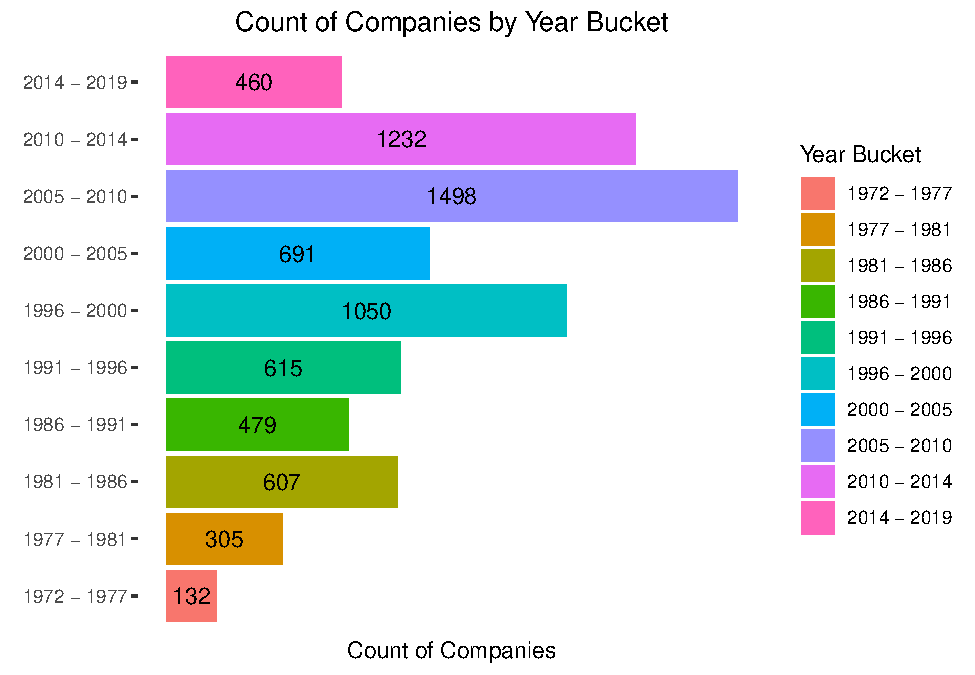
\includegraphics{Main_files/figure-latex/unnamed-chunk-8-1.pdf}

\hypertarget{and-so-now-i-know-that-most-of-my-value-is-in-the-time-period-that-goes-from-2005-to-2010.}{%
\subsection{And so, now I know that most of my value is in the time
period that goes from 2005 to
2010.}\label{and-so-now-i-know-that-most-of-my-value-is-in-the-time-period-that-goes-from-2005-to-2010.}}

\hypertarget{i-then-wanted-to-see-a-distribution-of-companies-by-employee-count.}{%
\subsection{I then wanted to see a distribution of companies by employee
count.}\label{i-then-wanted-to-see-a-distribution-of-companies-by-employee-count.}}

\hypertarget{but-first-i-wanted-to-see-if-we-had-any-nas-in-the-data-and-how-can-we-replace-them.}{%
\subsection{But first, I wanted to see if we had any NAs in the data,
and how can we replace
them.}\label{but-first-i-wanted-to-see-if-we-had-any-nas-in-the-data-and-how-can-we-replace-them.}}

\begin{Shaded}
\begin{Highlighting}[]
\NormalTok{dataset_emp <-}\StringTok{ }\NormalTok{dataset }\OperatorTok\StringTok{ }
\StringTok{  }\KeywordTok{select}\NormalTok{(EMPLOYEE_COUNT,COUNTRY) }\OperatorTok\StringTok{ }
\StringTok{  }\KeywordTok{filter}\NormalTok{(}\KeywordTok{is.na}\NormalTok{(EMPLOYEE_COUNT)) }\OperatorTok\StringTok{ }
\StringTok{  }\KeywordTok{count}\NormalTok{(COUNTRY)}

\NormalTok{dataset_emp}\OperatorTok{$}\NormalTok{COUNTRY <-}\StringTok{ }
\StringTok{  }\KeywordTok{factor}\NormalTok{(dataset_emp}\OperatorTok{$}\NormalTok{COUNTRY, }
         \DataTypeTok{levels =}\NormalTok{ dataset_emp}\OperatorTok{$}\NormalTok{COUNTRY[}\KeywordTok{order}\NormalTok{(dataset_emp}\OperatorTok{$}\NormalTok{n,}
                                            \DataTypeTok{decreasing =} \OtherTok{TRUE}\NormalTok{)])}

\NormalTok{dataset_emp }\OperatorTok\StringTok{ }
\StringTok{  }\KeywordTok{ggplot}\NormalTok{(}\KeywordTok{aes}\NormalTok{(}\DataTypeTok{x=}\NormalTok{COUNTRY,}
             \DataTypeTok{y=}\NormalTok{n,}
             \DataTypeTok{fill=}\KeywordTok{as.factor}\NormalTok{(n))}
\NormalTok{         )}\OperatorTok{+}
\StringTok{  }\KeywordTok{geom_col}\NormalTok{()}\OperatorTok{+}
\StringTok{  }\KeywordTok{ggtitle}\NormalTok{(}\StringTok{"Count of NAs Employee Count by Country"}\NormalTok{)}\OperatorTok{+}
\StringTok{  }\KeywordTok{theme}\NormalTok{(}\DataTypeTok{plot.title =} \KeywordTok{element_text}\NormalTok{(}\DataTypeTok{hjust =} \FloatTok{0.5}\NormalTok{),}
        \DataTypeTok{axis.text.x =} \KeywordTok{element_text}\NormalTok{(}\DataTypeTok{size =} \DecValTok{10}\NormalTok{,}
                                   \DataTypeTok{angle =} \DecValTok{90}\NormalTok{,}
                                   \DataTypeTok{hjust =} \FloatTok{.5}\NormalTok{,}
                                   \DataTypeTok{vjust =} \FloatTok{.5}\NormalTok{),}
        \DataTypeTok{panel.background =} \KeywordTok{element_blank}\NormalTok{()) }\OperatorTok{+}\StringTok{ }
\StringTok{  }\KeywordTok{ylab}\NormalTok{(}\KeywordTok{element_blank}\NormalTok{()) }\OperatorTok{+}
\StringTok{  }\KeywordTok{xlab}\NormalTok{(}\StringTok{"Country"}\NormalTok{) }\OperatorTok{+}
\StringTok{  }\KeywordTok{labs}\NormalTok{(}\DataTypeTok{fill =} \StringTok{"Count of NAs"}\NormalTok{)}
\end{Highlighting}
\end{Shaded}

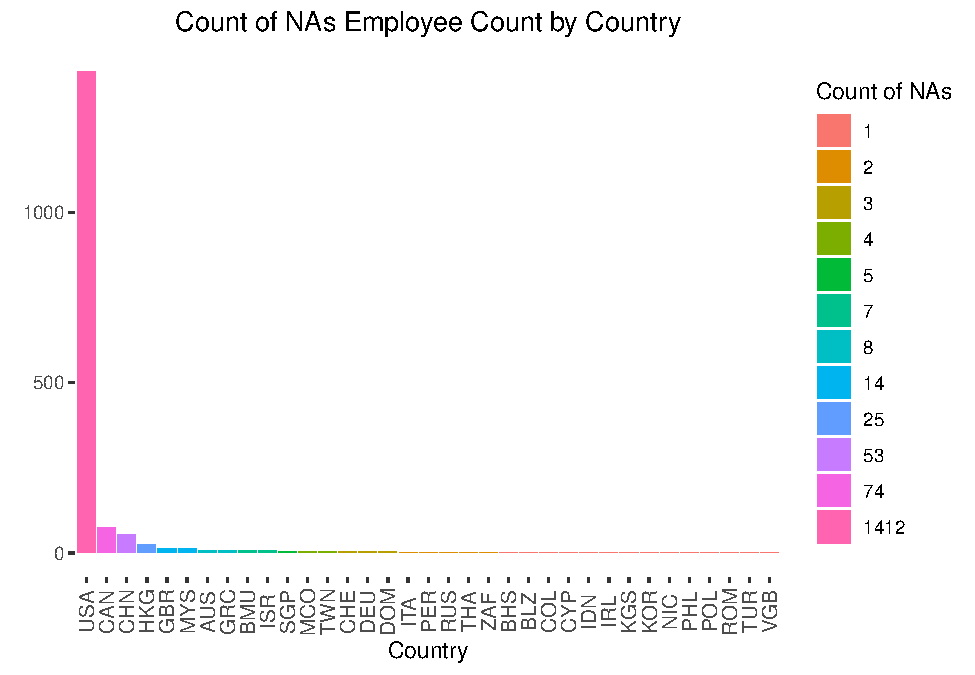
\includegraphics{Main_files/figure-latex/unnamed-chunk-9-1.pdf}

\hypertarget{unsurprisingly-usa-has-the-highest-amount-of-nas-which-correlates-with-it-having-the-highest-amount-of-companies}{%
\subsection{Unsurprisingly USA has the highest amount of NAs, which
correlates with it having the highest amount of
companies}\label{unsurprisingly-usa-has-the-highest-amount-of-nas-which-correlates-with-it-having-the-highest-amount-of-companies}}

\hypertarget{then-i-wanted-to-see-the-variance-of-employee-counts-of-all-countries-where-i-had-nas-but-where-i-had-no-na-values}{%
\subsection{Then I wanted to see the variance of Employee Counts, of all
countries where I had NAs, but where I had no NA
values}\label{then-i-wanted-to-see-the-variance-of-employee-counts-of-all-countries-where-i-had-nas-but-where-i-had-no-na-values}}

\begin{Shaded}
\begin{Highlighting}[]
\NormalTok{dataset_emp_noNA <-}\StringTok{ }
\NormalTok{dataset }\OperatorTok\StringTok{ }
\StringTok{  }\KeywordTok{select}\NormalTok{(EMPLOYEE_COUNT,COUNTRY) }\OperatorTok\StringTok{ }
\StringTok{  }\KeywordTok{filter}\NormalTok{(}\OperatorTok{!}\KeywordTok{is.na}\NormalTok{(EMPLOYEE_COUNT))}

\NormalTok{dataset_emp_noNA <-}\StringTok{ }
\StringTok{  }\KeywordTok{merge}\NormalTok{(dataset_emp_noNA }\OperatorTok\StringTok{ }
\StringTok{          }\KeywordTok{select}\NormalTok{(COUNTRY,EMPLOYEE_COUNT),}
\NormalTok{        dataset_emp }\OperatorTok\StringTok{ }
\StringTok{          }\KeywordTok{select}\NormalTok{(COUNTRY),}\DataTypeTok{all=}\OtherTok{FALSE}\NormalTok{)}

\NormalTok{dataset_emp_noNA }\OperatorTok\StringTok{ }
\StringTok{  }\KeywordTok{ggplot}\NormalTok{(}\KeywordTok{aes}\NormalTok{(}\DataTypeTok{x=}\NormalTok{COUNTRY,}\DataTypeTok{y=}\NormalTok{EMPLOYEE_COUNT))}\OperatorTok{+}
\StringTok{  }\KeywordTok{geom_boxplot}\NormalTok{()}\OperatorTok{+}
\StringTok{  }\KeywordTok{ggtitle}\NormalTok{(}\StringTok{"Variance of Employee Count by Country"}\NormalTok{)}\OperatorTok{+}
\StringTok{  }\KeywordTok{theme}\NormalTok{(}\DataTypeTok{plot.title =} \KeywordTok{element_text}\NormalTok{(}\DataTypeTok{hjust =} \FloatTok{0.5}\NormalTok{),}
        \DataTypeTok{axis.text.x =} \KeywordTok{element_text}\NormalTok{(}\DataTypeTok{size =} \DecValTok{10}\NormalTok{,}
                                   \DataTypeTok{angle =} \DecValTok{90}\NormalTok{,}
                                   \DataTypeTok{hjust =} \FloatTok{.5}\NormalTok{,}
                                   \DataTypeTok{vjust =} \FloatTok{.5}\NormalTok{),}
        \DataTypeTok{panel.background =} \KeywordTok{element_blank}\NormalTok{()) }\OperatorTok{+}
\StringTok{  }\KeywordTok{ylab}\NormalTok{(}\StringTok{"Employee Count"}\NormalTok{) }\OperatorTok{+}\StringTok{ }
\StringTok{  }\KeywordTok{xlab}\NormalTok{(}\StringTok{"Country"}\NormalTok{)}
\end{Highlighting}
\end{Shaded}

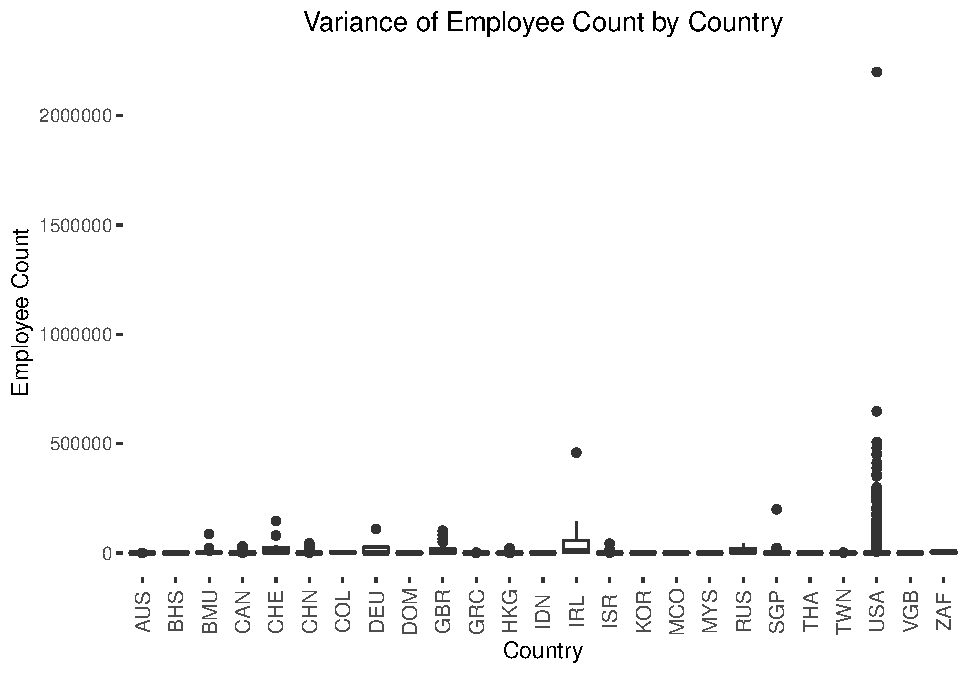
\includegraphics{Main_files/figure-latex/unnamed-chunk-10-1.pdf}

\hypertarget{with-this-data-i-decided-that-the-best-way-to-replace-the-nas-was-to-use-the-median-by-country.}{%
\subsection{With this data, I decided that the best way to replace the
NAs, was to use the median by
country.}\label{with-this-data-i-decided-that-the-best-way-to-replace-the-nas-was-to-use-the-median-by-country.}}

\hypertarget{the-reason-behind-this-is-because-of-the-outliers-in-the-data-means-we-can-use-the-median-as-better-measure.}{%
\subsection{The reason behind this is because of the outliers in the
data, means we can use the median as better
measure.}\label{the-reason-behind-this-is-because-of-the-outliers-in-the-data-means-we-can-use-the-median-as-better-measure.}}

\begin{Shaded}
\begin{Highlighting}[]
\ControlFlowTok{for}\NormalTok{ (country }\ControlFlowTok{in} \KeywordTok{unique}\NormalTok{(dataset}\OperatorTok{$}\NormalTok{COUNTRY))\{}
  
\NormalTok{  dataset_fil <-}
\StringTok{    }\NormalTok{dataset }\OperatorTok\StringTok{ }
\StringTok{    }\KeywordTok{filter}\NormalTok{(}\OperatorTok{!}\KeywordTok{is.na}\NormalTok{(EMPLOYEE_COUNT)) }\OperatorTok\StringTok{ }
\StringTok{    }\KeywordTok{filter}\NormalTok{(COUNTRY }\OperatorTok{==}\StringTok{ }\NormalTok{country)}
  
\NormalTok{  dataset}\OperatorTok{$}\NormalTok{EMPLOYEE_COUNT <-}\StringTok{ }
\StringTok{    }\KeywordTok{replace_na}\NormalTok{(dataset}\OperatorTok{$}\NormalTok{EMPLOYEE_COUNT,}
               \KeywordTok{quantile}\NormalTok{(}\KeywordTok{na.exclude}\NormalTok{(dataset_fil}\OperatorTok{$}\NormalTok{EMPLOYEE_COUNT),}
                        \DataTypeTok{probs=}\FloatTok{0.5}\NormalTok{))}
\NormalTok{\}}

\KeywordTok{summary}\NormalTok{(dataset)}
\end{Highlighting}
\end{Shaded}

\begin{verbatim}
##                                COMPANY_NAME         CITY     
##  024 Pharma Inc                      :   1   New York : 473  
##  1-800 Flowers.com, Inc.             :   1   Houston  : 262  
##  10x Genomics Inc                    :   1   Las Vegas: 188  
##  11 Good Energy Inc                  :   1   Dallas   : 130  
##  1347 Property Insurance Holdings Inc:   1   San Diego: 109  
##  180 Degree Capital Corp             :   1   (Other)  :7117  
##  (Other)                             :8376   NA's     : 103  
##      STATE           ZIP          COUNTRY              PHONE     
##  CA     :1280   10022  :  84   USA    :7283   800 983-0903:  11  
##  NY     : 739   77002  :  67   CHN    : 308   855 588-7839:   8  
##  TX     : 733   92121  :  47   CAN    : 205   510 522-9600:   7  
##  FL     : 553   80202  :  43   HKG    :  91   512 236-6555:   6  
##  NV     : 315   10019  :  36   ISR    :  80   800 736-3402:   6  
##  (Other):4175   (Other):7968   (Other): 414   (Other)     :8310  
##  NA's   : 587   NA's   : 137   NA's   :   1   NA's        :  34  
##   YEAR_INCORP    ANNUAL_SALES        EMPLOYEE_COUNT   
##  Min.   :1784   Min.   :-2.781e+08   Min.   :      0  
##  1st Qu.:1986   1st Qu.: 4.095e+06   1st Qu.:     28  
##  Median :1999   Median : 8.760e+07   Median :    207  
##  Mean   :1991   Mean   : 2.709e+09   Mean   :   5385  
##  3rd Qu.:2008   3rd Qu.: 9.903e+08   3rd Qu.:   1177  
##  Max.   :2019   Max.   : 5.144e+11   Max.   :2200000  
##  NA's   :157    NA's   :1625                          
##    NET_INCOME              YEAR_BUCKET  
##  Min.   :-2.244e+10   1996 - 2019:4931  
##  1st Qu.:-5.216e+06   1972 - 1996:2107  
##  Median :-7.610e+04   1948 - 1972: 567  
##  Mean   : 1.758e+08   1925 - 1948: 229  
##  3rd Qu.: 2.798e+07   1902 - 1925: 221  
##  Max.   : 5.953e+10   (Other)    : 170  
##  NA's   :25           NA's       : 157
\end{verbatim}

\hypertarget{with-this-summary-i-wanted-to-check-the-new-values-of-the-employee-count-column}{%
\subsection{With this summary I wanted to check the new values of the
Employee Count
column}\label{with-this-summary-i-wanted-to-check-the-new-values-of-the-employee-count-column}}

\hypertarget{i-decided-to-use-the-same-approach-as-before-where-i-created-buckets-to-see-the-distribution}{%
\subsection{I decided to use the same approach as before, where I
created buckets to see the
distribution}\label{i-decided-to-use-the-same-approach-as-before-where-i-created-buckets-to-see-the-distribution}}

\begin{Shaded}
\begin{Highlighting}[]
\NormalTok{dataset}\OperatorTok{$}\NormalTok{EMPLOYEE_COUNT_BUCKET <-}\StringTok{ }\KeywordTok{cut}\NormalTok{(dataset}\OperatorTok{$}\NormalTok{EMPLOYEE_COUNT,}\DataTypeTok{breaks =} \DecValTok{20}\NormalTok{,}\DataTypeTok{dig.lab =} \DecValTok{10}\NormalTok{)}
\NormalTok{dataset}\OperatorTok{$}\NormalTok{EMPLOYEE_COUNT_BUCKET <-}\StringTok{ }\KeywordTok{str_replace}\NormalTok{(dataset}\OperatorTok{$}\NormalTok{EMPLOYEE_COUNT_BUCKET, }\StringTok{"}\CharTok{\textbackslash{}\textbackslash{}}\StringTok{("}\NormalTok{, }\StringTok{""}\NormalTok{)}
\NormalTok{dataset}\OperatorTok{$}\NormalTok{EMPLOYEE_COUNT_BUCKET <-}\StringTok{ }\KeywordTok{str_replace}\NormalTok{(dataset}\OperatorTok{$}\NormalTok{EMPLOYEE_COUNT_BUCKET, }\StringTok{"]"}\NormalTok{, }\StringTok{""}\NormalTok{)}
\NormalTok{dataset}\OperatorTok{$}\NormalTok{EMPLOYEE_COUNT_BUCKET <-}\StringTok{ }\KeywordTok{str_replace}\NormalTok{(dataset}\OperatorTok{$}\NormalTok{EMPLOYEE_COUNT_BUCKET, }\StringTok{","}\NormalTok{, }\StringTok{" - "}\NormalTok{)}
\NormalTok{dataset}\OperatorTok{$}\NormalTok{EMPLOYEE_COUNT_BUCKET <-}\StringTok{ }\KeywordTok{str_replace}\NormalTok{(dataset}\OperatorTok{$}\NormalTok{EMPLOYEE_COUNT_BUCKET, }\StringTok{"-2200"}\NormalTok{, }\StringTok{"0"}\NormalTok{)}

\NormalTok{dataset}\OperatorTok{$}\NormalTok{EMPLOYEE_COUNT_BUCKET <-}\StringTok{ }\KeywordTok{as.factor}\NormalTok{(dataset}\OperatorTok{$}\NormalTok{EMPLOYEE_COUNT_BUCKET)}

\KeywordTok{summary}\NormalTok{(dataset)}
\end{Highlighting}
\end{Shaded}

\begin{verbatim}
##                                COMPANY_NAME         CITY     
##  024 Pharma Inc                      :   1   New York : 473  
##  1-800 Flowers.com, Inc.             :   1   Houston  : 262  
##  10x Genomics Inc                    :   1   Las Vegas: 188  
##  11 Good Energy Inc                  :   1   Dallas   : 130  
##  1347 Property Insurance Holdings Inc:   1   San Diego: 109  
##  180 Degree Capital Corp             :   1   (Other)  :7117  
##  (Other)                             :8376   NA's     : 103  
##      STATE           ZIP          COUNTRY              PHONE     
##  CA     :1280   10022  :  84   USA    :7283   800 983-0903:  11  
##  NY     : 739   77002  :  67   CHN    : 308   855 588-7839:   8  
##  TX     : 733   92121  :  47   CAN    : 205   510 522-9600:   7  
##  FL     : 553   80202  :  43   HKG    :  91   512 236-6555:   6  
##  NV     : 315   10019  :  36   ISR    :  80   800 736-3402:   6  
##  (Other):4175   (Other):7968   (Other): 414   (Other)     :8310  
##  NA's   : 587   NA's   : 137   NA's   :   1   NA's        :  34  
##   YEAR_INCORP    ANNUAL_SALES        EMPLOYEE_COUNT   
##  Min.   :1784   Min.   :-2.781e+08   Min.   :      0  
##  1st Qu.:1986   1st Qu.: 4.095e+06   1st Qu.:     28  
##  Median :1999   Median : 8.760e+07   Median :    207  
##  Mean   :1991   Mean   : 2.709e+09   Mean   :   5385  
##  3rd Qu.:2008   3rd Qu.: 9.903e+08   3rd Qu.:   1177  
##  Max.   :2019   Max.   : 5.144e+11   Max.   :2200000  
##  NA's   :157    NA's   :1625                          
##    NET_INCOME              YEAR_BUCKET         EMPLOYEE_COUNT_BUCKET
##  Min.   :-2.244e+10   1996 - 2019:4931   0 - 110000       :8315     
##  1st Qu.:-5.216e+06   1972 - 1996:2107   110000 - 220000  :  37     
##  Median :-7.610e+04   1948 - 1972: 567   2090000 - 2202200:   1     
##  Mean   : 1.758e+08   1925 - 1948: 229   220000 - 330000  :  18     
##  3rd Qu.: 2.798e+07   1902 - 1925: 221   330000 - 440000  :   5     
##  Max.   : 5.953e+10   (Other)    : 170   440000 - 550000  :   5     
##  NA's   :25           NA's       : 157   550000 - 660000  :   1
\end{verbatim}

\hypertarget{with-this-summary-i-wanted-to-check-the-employee-count-bucket-column}{%
\subsection{With this summary I wanted to check the Employee Count
Bucket
column}\label{with-this-summary-i-wanted-to-check-the-employee-count-bucket-column}}

\hypertarget{and-with-the-graphic-i-realized-that-most-companies-have-between-0-and-110000-employees.}{%
\subsection{And with the graphic, I realized that most companies have
between 0 and 110,000
employees.}\label{and-with-the-graphic-i-realized-that-most-companies-have-between-0-and-110000-employees.}}

\begin{Shaded}
\begin{Highlighting}[]
\KeywordTok{ggplot}\NormalTok{(dataset }\OperatorTok
\StringTok{  }\KeywordTok{count}\NormalTok{(EMPLOYEE_COUNT_BUCKET),}
  \KeywordTok{aes}\NormalTok{(}\DataTypeTok{x =}\NormalTok{ EMPLOYEE_COUNT_BUCKET,}
      \DataTypeTok{y=}\NormalTok{n,}
      \DataTypeTok{fill=}\NormalTok{EMPLOYEE_COUNT_BUCKET))}\OperatorTok{+}
\StringTok{  }\KeywordTok{geom_col}\NormalTok{()}\OperatorTok{+}
\StringTok{  }\KeywordTok{geom_text}\NormalTok{(}\KeywordTok{aes}\NormalTok{(}\DataTypeTok{label =}\NormalTok{ n),}\DataTypeTok{position =} \KeywordTok{position_stack}\NormalTok{(}\DataTypeTok{vjust =} \FloatTok{.5}\NormalTok{)) }\OperatorTok{+}
\StringTok{  }\KeywordTok{ggtitle}\NormalTok{(}\StringTok{"Count of Companies by Employee Number Bucket"}\NormalTok{)}\OperatorTok{+}
\StringTok{  }\KeywordTok{theme}\NormalTok{(}\DataTypeTok{plot.title =} \KeywordTok{element_text}\NormalTok{(}\DataTypeTok{hjust =} \FloatTok{0.5}\NormalTok{),}
        \DataTypeTok{axis.text.x =} \KeywordTok{element_blank}\NormalTok{(),}
        \DataTypeTok{axis.ticks.x =} \KeywordTok{element_blank}\NormalTok{(),}
        \DataTypeTok{panel.background =} \KeywordTok{element_blank}\NormalTok{())}\OperatorTok{+}
\StringTok{  }\KeywordTok{ylab}\NormalTok{(}\StringTok{"Count of Companies"}\NormalTok{) }\OperatorTok{+}
\StringTok{  }\KeywordTok{xlab}\NormalTok{(}\KeywordTok{element_blank}\NormalTok{()) }\OperatorTok{+}
\StringTok{  }\KeywordTok{labs}\NormalTok{(}\DataTypeTok{fill =} \StringTok{"Employee Number Bucket"}\NormalTok{) }\OperatorTok{+}
\StringTok{  }\KeywordTok{coord_flip}\NormalTok{()}
\end{Highlighting}
\end{Shaded}

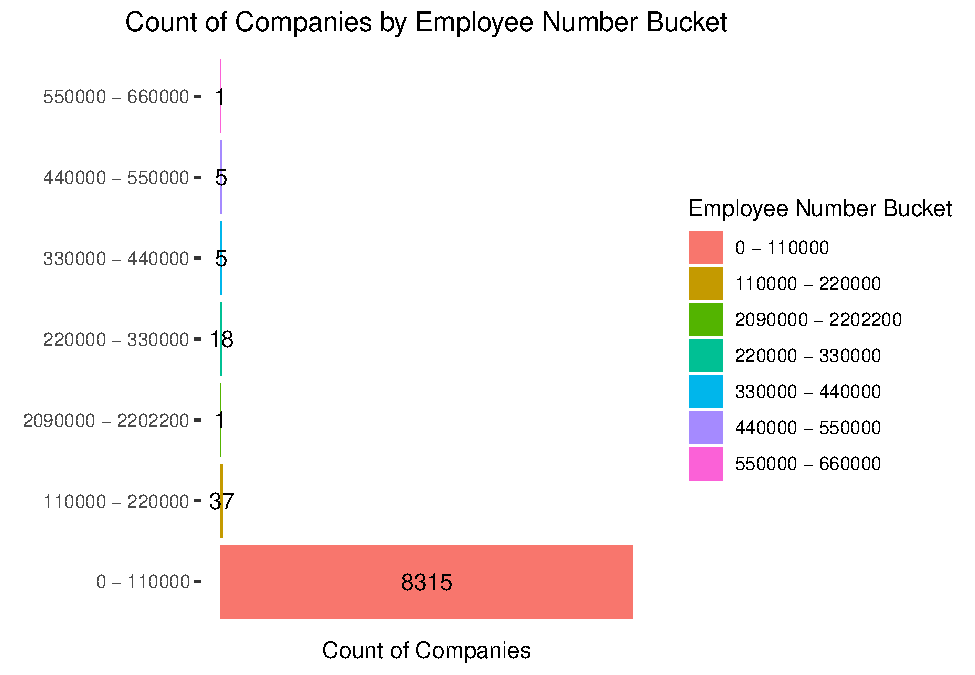
\includegraphics{Main_files/figure-latex/unnamed-chunk-13-1.pdf}

\hypertarget{as-a-third-point-i-wanted-to-see-the-distribution-by-country.}{%
\subsection{As a third point, I wanted to see the distribution by
Country.}\label{as-a-third-point-i-wanted-to-see-the-distribution-by-country.}}

\hypertarget{this-distribution-sounds-easy-enough-but-again-the-graphic-shows-otherwise.}{%
\subsection{This distribution sounds easy enough, but again, the graphic
shows
otherwise.}\label{this-distribution-sounds-easy-enough-but-again-the-graphic-shows-otherwise.}}

\begin{Shaded}
\begin{Highlighting}[]
\KeywordTok{ggplot}\NormalTok{(dataset }\OperatorTok\StringTok{ }
\StringTok{         }\KeywordTok{count}\NormalTok{(COUNTRY),}
       \KeywordTok{aes}\NormalTok{(}\DataTypeTok{x=}\NormalTok{COUNTRY,}
           \DataTypeTok{y=}\NormalTok{n,}
           \DataTypeTok{fill=}\NormalTok{COUNTRY))}\OperatorTok{+}
\StringTok{  }\KeywordTok{geom_col}\NormalTok{()}\OperatorTok{+}
\StringTok{  }\KeywordTok{geom_text}\NormalTok{(}\KeywordTok{aes}\NormalTok{(}\DataTypeTok{label =}\NormalTok{ n),}\DataTypeTok{position =} \KeywordTok{position_stack}\NormalTok{(}\DataTypeTok{vjust =} \FloatTok{.5}\NormalTok{)) }\OperatorTok{+}
\StringTok{  }\KeywordTok{ggtitle}\NormalTok{(}\StringTok{"Count of Companies by Country"}\NormalTok{)}\OperatorTok{+}
\StringTok{  }\KeywordTok{theme}\NormalTok{(}\DataTypeTok{plot.title =} \KeywordTok{element_text}\NormalTok{(}\DataTypeTok{hjust =} \FloatTok{0.5}\NormalTok{),}
        \DataTypeTok{axis.text.x =} \KeywordTok{element_blank}\NormalTok{(),}
        \DataTypeTok{axis.ticks.x =} \KeywordTok{element_blank}\NormalTok{(),}
        \DataTypeTok{panel.background =} \KeywordTok{element_blank}\NormalTok{())}\OperatorTok{+}
\StringTok{  }\KeywordTok{ylab}\NormalTok{(}\StringTok{"Count of Companies"}\NormalTok{) }\OperatorTok{+}
\StringTok{  }\KeywordTok{xlab}\NormalTok{(}\KeywordTok{element_blank}\NormalTok{()) }\OperatorTok{+}
\StringTok{  }\KeywordTok{labs}\NormalTok{(}\DataTypeTok{fill =} \StringTok{"Country"}\NormalTok{) }\OperatorTok{+}
\StringTok{  }\KeywordTok{coord_flip}\NormalTok{()}
\end{Highlighting}
\end{Shaded}

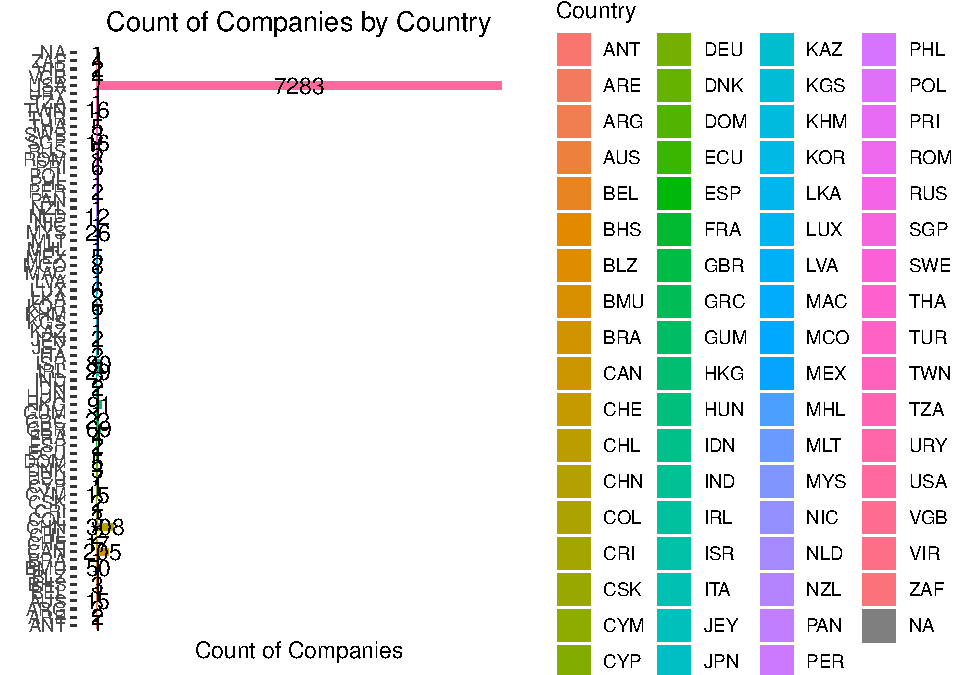
\includegraphics{Main_files/figure-latex/unnamed-chunk-14-1.pdf}

\hypertarget{what-i-decided-for-this-distribution-and-since-we-have-way-too-many-countries-was-that-i-wanted-to-see-the-top-countries}{%
\subsection{What I decided for this distribution, and since we have way
too many countries, was that I wanted to see the top
countries}\label{what-i-decided-for-this-distribution-and-since-we-have-way-too-many-countries-was-that-i-wanted-to-see-the-top-countries}}

\hypertarget{so-i-did-the-distribution-ordered-the-results-by-number-of-companies-and-then-took-the-top-10-companies}{%
\subsection{So I did the distribution, ordered the results by number of
companies, and then took the top 10
companies}\label{so-i-did-the-distribution-ordered-the-results-by-number-of-companies-and-then-took-the-top-10-companies}}

\begin{Shaded}
\begin{Highlighting}[]
\NormalTok{dataset_country <-}\StringTok{ }\NormalTok{dataset }\OperatorTok\StringTok{ }\KeywordTok{filter}\NormalTok{(}\OperatorTok{!}\KeywordTok{is.na}\NormalTok{(COUNTRY))}

\NormalTok{dataset_country_}\DecValTok{2}\NormalTok{ <-}\StringTok{ }\NormalTok{dataset_country }\OperatorTok\StringTok{ }\KeywordTok{count}\NormalTok{(COUNTRY)}

\NormalTok{dataset_country_f <-}\StringTok{ }\KeywordTok{tail}\NormalTok{(dataset_country_}\DecValTok{2}\NormalTok{[}\KeywordTok{order}\NormalTok{(dataset_country_}\DecValTok{2}\OperatorTok{$}\NormalTok{n),],}\DecValTok{10}\NormalTok{)}

\NormalTok{dataset_country_f}\OperatorTok{$}\NormalTok{COUNTRY <-}\StringTok{ }
\StringTok{  }\KeywordTok{factor}\NormalTok{(dataset_country_f}\OperatorTok{$}\NormalTok{COUNTRY,}
         \DataTypeTok{levels =}\NormalTok{ dataset_country_f}\OperatorTok{$}\NormalTok{COUNTRY[}\KeywordTok{order}\NormalTok{(dataset_country_f}\OperatorTok{$}\NormalTok{n)])}

\KeywordTok{ggplot}\NormalTok{(dataset_country_f,}\KeywordTok{aes}\NormalTok{(}\DataTypeTok{x=}\NormalTok{COUNTRY,}\DataTypeTok{y=}\NormalTok{n,}\DataTypeTok{fill=}\NormalTok{COUNTRY))}\OperatorTok{+}
\StringTok{  }\KeywordTok{geom_col}\NormalTok{()}\OperatorTok{+}
\StringTok{  }\KeywordTok{geom_text}\NormalTok{(}\KeywordTok{aes}\NormalTok{(}\DataTypeTok{label =}\NormalTok{ n),}\DataTypeTok{position =} \KeywordTok{position_stack}\NormalTok{(}\DataTypeTok{vjust =} \FloatTok{.5}\NormalTok{)) }\OperatorTok{+}
\StringTok{  }\KeywordTok{ggtitle}\NormalTok{(}\StringTok{"Count of Companies by Country"}\NormalTok{)}\OperatorTok{+}
\StringTok{  }\KeywordTok{theme}\NormalTok{(}\DataTypeTok{plot.title =} \KeywordTok{element_text}\NormalTok{(}\DataTypeTok{hjust =} \FloatTok{0.5}\NormalTok{),}
        \DataTypeTok{axis.text.x =} \KeywordTok{element_blank}\NormalTok{(),}
        \DataTypeTok{axis.ticks.x =} \KeywordTok{element_blank}\NormalTok{(),}
        \DataTypeTok{panel.background =} \KeywordTok{element_blank}\NormalTok{())}\OperatorTok{+}
\StringTok{  }\KeywordTok{ylab}\NormalTok{(}\StringTok{"Count of Companies"}\NormalTok{) }\OperatorTok{+}
\StringTok{  }\KeywordTok{xlab}\NormalTok{(}\KeywordTok{element_blank}\NormalTok{()) }\OperatorTok{+}
\StringTok{  }\KeywordTok{labs}\NormalTok{(}\DataTypeTok{fill =} \StringTok{"Country"}\NormalTok{) }\OperatorTok{+}
\StringTok{  }\KeywordTok{coord_flip}\NormalTok{()}
\end{Highlighting}
\end{Shaded}

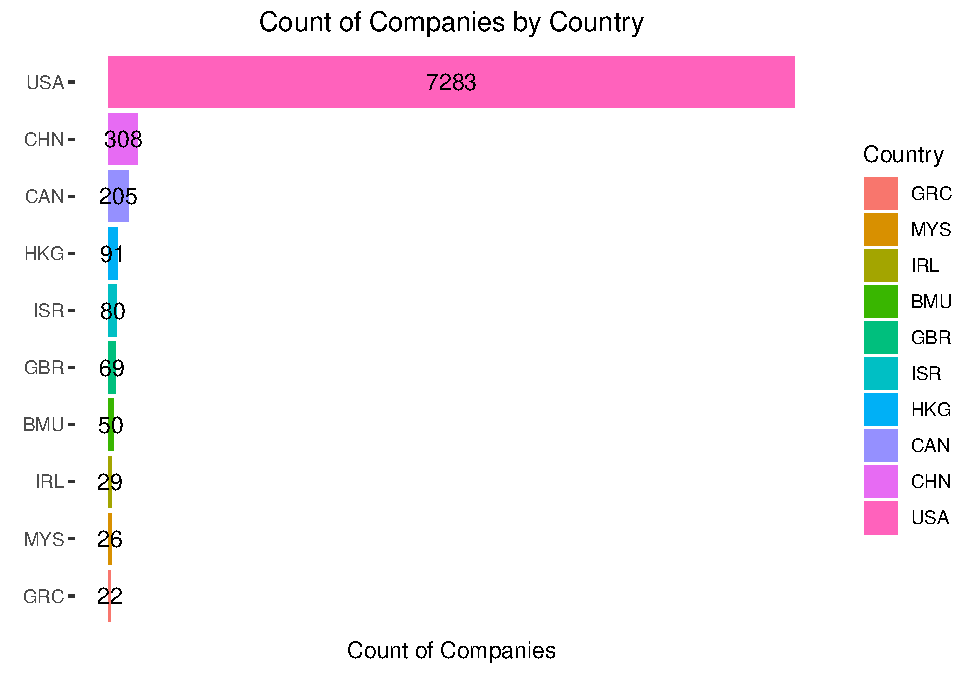
\includegraphics{Main_files/figure-latex/unnamed-chunk-15-1.pdf}

\hypertarget{unsurprinsingly-usa-is-the-top-country.}{%
\subsection{Unsurprinsingly, USA is the top
country.}\label{unsurprinsingly-usa-is-the-top-country.}}

\hypertarget{what-is-noteworthy-is-that-the-rest-of-the-coutries-have-less-than-5-of-the-companies-that-usa-has.}{%
\subsection{What is noteworthy, is that the rest of the coutries have
less than 5\% of the companies that USA
has.}\label{what-is-noteworthy-is-that-the-rest-of-the-coutries-have-less-than-5-of-the-companies-that-usa-has.}}

\hypertarget{now-i-want-to-see-the-annual-sales-during-the-year-where-most-companies-where-incorporated.}{%
\subsection{Now I want to see the annual sales during the year where
most companies where
incorporated.}\label{now-i-want-to-see-the-annual-sales-during-the-year-where-most-companies-where-incorporated.}}

\begin{Shaded}
\begin{Highlighting}[]
\KeywordTok{ggplot}\NormalTok{(dataset }\OperatorTok
\StringTok{         }\KeywordTok{filter}\NormalTok{(YEAR_INCORP }\OperatorTok{>}\StringTok{ }\DecValTok{2000}\NormalTok{) }\OperatorTok\StringTok{ }
\StringTok{         }\KeywordTok{count}\NormalTok{(YEAR_INCORP),}
       \KeywordTok{aes}\NormalTok{(}\DataTypeTok{x=}\NormalTok{YEAR_INCORP,}
           \DataTypeTok{y=}\NormalTok{n,}
           \DataTypeTok{fill=}\KeywordTok{as.factor}\NormalTok{(YEAR_INCORP))) }\OperatorTok{+}
\StringTok{  }\KeywordTok{geom_col}\NormalTok{()}\OperatorTok{+}
\StringTok{  }\KeywordTok{geom_text}\NormalTok{(}\KeywordTok{aes}\NormalTok{(}\DataTypeTok{label =}\NormalTok{ n),}\DataTypeTok{position =} \KeywordTok{position_stack}\NormalTok{(}\DataTypeTok{vjust =} \FloatTok{.5}\NormalTok{), }\DataTypeTok{size =} \FloatTok{3.5}\NormalTok{) }\OperatorTok{+}
\StringTok{  }\KeywordTok{ggtitle}\NormalTok{(}\StringTok{"Count of Companies by Year"}\NormalTok{)}\OperatorTok{+}
\StringTok{  }\KeywordTok{theme}\NormalTok{(}\DataTypeTok{plot.title =} \KeywordTok{element_text}\NormalTok{(}\DataTypeTok{hjust =} \FloatTok{0.5}\NormalTok{),}
        \CommentTok{#axis.text.x = element_blank(),}
        \CommentTok{#axis.ticks.x = element_blank(),}
        \DataTypeTok{panel.background =} \KeywordTok{element_blank}\NormalTok{())}\OperatorTok{+}
\StringTok{  }\KeywordTok{ylab}\NormalTok{(}\StringTok{"Count of Companies"}\NormalTok{) }\OperatorTok{+}
\StringTok{  }\KeywordTok{xlab}\NormalTok{(}\KeywordTok{element_blank}\NormalTok{()) }\OperatorTok{+}
\StringTok{  }\KeywordTok{labs}\NormalTok{(}\DataTypeTok{fill =} \StringTok{"Year"}\NormalTok{) }\OperatorTok{+}
\StringTok{  }\KeywordTok{coord_flip}\NormalTok{()}
\end{Highlighting}
\end{Shaded}

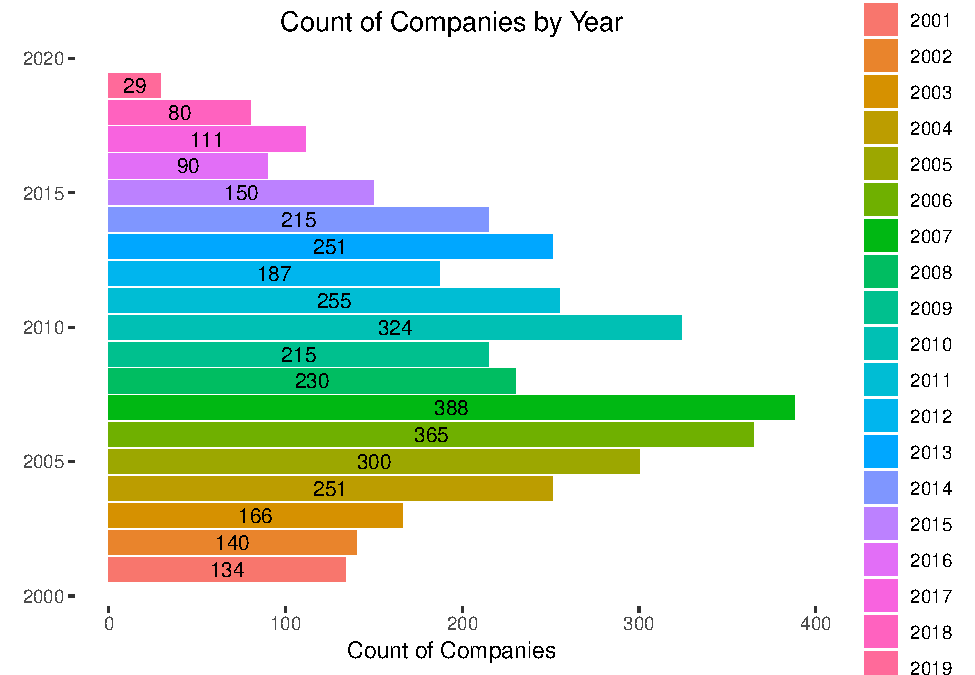
\includegraphics{Main_files/figure-latex/unnamed-chunk-16-1.pdf}

\hypertarget{with-this-i-can-see-that-2007-is-the-year-where-the-most-companies-where-incorporated.}{%
\subsection{With this, I can see that 2007 is the year where the most
companies where
incorporated.}\label{with-this-i-can-see-that-2007-is-the-year-where-the-most-companies-where-incorporated.}}

\hypertarget{ww-knew-to-look-into-this-time-period-because-of-the-previous-bucket-analysis}{%
\subsection{Ww knew to look into this time period because of the
previous bucket
analysis}\label{ww-knew-to-look-into-this-time-period-because-of-the-previous-bucket-analysis}}

\hypertarget{however-before-doing-the-analysis-we-need-to-replace-the-nas-in-the-dataset}{%
\subsection{However, before doing the analysis, we need to replace the
NAs in the
dataset}\label{however-before-doing-the-analysis-we-need-to-replace-the-nas-in-the-dataset}}

\hypertarget{we-can-check-the-variance-of-the-countries-in-the-same-way-we-did-before.}{%
\subsection{We can check the variance of the countries, in the same way
we did
before.}\label{we-can-check-the-variance-of-the-countries-in-the-same-way-we-did-before.}}

\begin{Shaded}
\begin{Highlighting}[]
\KeywordTok{options}\NormalTok{(}\DataTypeTok{scipen =} \DecValTok{999}\NormalTok{)}

\NormalTok{dataset_annsl <-}\StringTok{ }\NormalTok{dataset }\OperatorTok\StringTok{ }
\StringTok{  }\KeywordTok{select}\NormalTok{(ANNUAL_SALES,COUNTRY) }\OperatorTok
\StringTok{  }\KeywordTok{filter}\NormalTok{(}\KeywordTok{is.na}\NormalTok{(ANNUAL_SALES)) }\OperatorTok\StringTok{ }
\StringTok{  }\KeywordTok{count}\NormalTok{(COUNTRY)}

\NormalTok{dataset_annsl_noNA<-dataset }\OperatorTok\StringTok{ }
\StringTok{  }\KeywordTok{select}\NormalTok{(ANNUAL_SALES,COUNTRY) }\OperatorTok\StringTok{ }
\StringTok{  }\KeywordTok{filter}\NormalTok{(}\OperatorTok{!}\KeywordTok{is.na}\NormalTok{(ANNUAL_SALES))}

\NormalTok{dataset_annsl_noNA <-}\StringTok{ }\KeywordTok{merge}\NormalTok{(dataset_annsl_noNA }\OperatorTok\StringTok{ }
\StringTok{                              }\KeywordTok{select}\NormalTok{(COUNTRY,ANNUAL_SALES),}
\NormalTok{                            dataset_annsl }\OperatorTok\StringTok{ }
\StringTok{                              }\KeywordTok{select}\NormalTok{(COUNTRY),}\DataTypeTok{all=}\OtherTok{FALSE}\NormalTok{)}

\NormalTok{dataset_annsl_noNA }\OperatorTok\StringTok{ }\KeywordTok{ggplot}\NormalTok{(}\KeywordTok{aes}\NormalTok{(}\DataTypeTok{x=}\NormalTok{COUNTRY,}
                                  \DataTypeTok{y=}\NormalTok{ANNUAL_SALES))}\OperatorTok{+}
\StringTok{  }\KeywordTok{geom_boxplot}\NormalTok{()}\OperatorTok{+}
\StringTok{  }\KeywordTok{ggtitle}\NormalTok{(}\StringTok{"Variance of Annual Sales by Country"}\NormalTok{)}\OperatorTok{+}
\StringTok{  }\KeywordTok{theme}\NormalTok{(}\DataTypeTok{axis.text.x =} \KeywordTok{element_text}\NormalTok{(}\DataTypeTok{size =} \DecValTok{10}\NormalTok{, }\DataTypeTok{angle =} \DecValTok{90}\NormalTok{, }\DataTypeTok{hjust =} \FloatTok{.5}\NormalTok{, }\DataTypeTok{vjust =} \FloatTok{.5}\NormalTok{),}
        \DataTypeTok{panel.background =} \KeywordTok{element_blank}\NormalTok{(),}
        \DataTypeTok{plot.title =} \KeywordTok{element_text}\NormalTok{(}\DataTypeTok{hjust =} \FloatTok{0.5}\NormalTok{)) }\OperatorTok{+}
\StringTok{  }\KeywordTok{ylab}\NormalTok{(}\StringTok{"Annual Sales"}\NormalTok{) }\OperatorTok{+}\StringTok{ }
\StringTok{  }\KeywordTok{xlab}\NormalTok{(}\StringTok{"Country"}\NormalTok{)}
\end{Highlighting}
\end{Shaded}

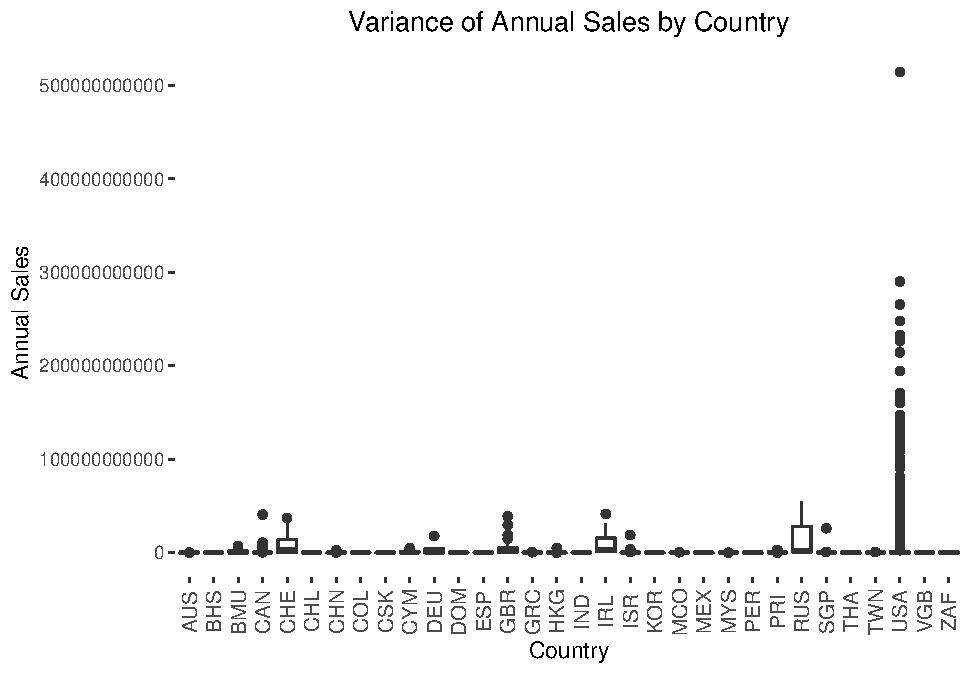
\includegraphics{Main_files/figure-latex/unnamed-chunk-17-1.pdf}

\hypertarget{and-as-before-im-using-the-median-for-each-country}{%
\subsection{And, as before, I'm using the median for each
country}\label{and-as-before-im-using-the-median-for-each-country}}

\begin{Shaded}
\begin{Highlighting}[]
\ControlFlowTok{for}\NormalTok{ (country }\ControlFlowTok{in} \KeywordTok{unique}\NormalTok{(dataset}\OperatorTok{$}\NormalTok{COUNTRY))\{}
\NormalTok{  dataset_fil <-}\StringTok{ }\NormalTok{dataset }\OperatorTok\StringTok{ }
\StringTok{    }\KeywordTok{filter}\NormalTok{(}\OperatorTok{!}\KeywordTok{is.na}\NormalTok{(ANNUAL_SALES)) }\OperatorTok
\StringTok{    }\KeywordTok{filter}\NormalTok{(COUNTRY }\OperatorTok{==}\StringTok{ }\NormalTok{country)}
\NormalTok{  dataset}\OperatorTok{$}\NormalTok{ANNUAL_SALES <-}\StringTok{ }\KeywordTok{replace_na}\NormalTok{(dataset}\OperatorTok{$}\NormalTok{ANNUAL_SALES,}
                                     \KeywordTok{quantile}\NormalTok{(}\KeywordTok{na.exclude}\NormalTok{(dataset_fil}\OperatorTok{$}\NormalTok{ANNUAL_SALES),}
                                              \DataTypeTok{probs=}\FloatTok{0.5}\NormalTok{))}
\NormalTok{\}}

\KeywordTok{summary}\NormalTok{(dataset)}
\end{Highlighting}
\end{Shaded}

\begin{verbatim}
##                                COMPANY_NAME         CITY     
##  024 Pharma Inc                      :   1   New York : 473  
##  1-800 Flowers.com, Inc.             :   1   Houston  : 262  
##  10x Genomics Inc                    :   1   Las Vegas: 188  
##  11 Good Energy Inc                  :   1   Dallas   : 130  
##  1347 Property Insurance Holdings Inc:   1   San Diego: 109  
##  180 Degree Capital Corp             :   1   (Other)  :7117  
##  (Other)                             :8376   NA's     : 103  
##      STATE           ZIP          COUNTRY              PHONE     
##  CA     :1280   10022  :  84   USA    :7283   800 983-0903:  11  
##  NY     : 739   77002  :  67   CHN    : 308   855 588-7839:   8  
##  TX     : 733   92121  :  47   CAN    : 205   510 522-9600:   7  
##  FL     : 553   80202  :  43   HKG    :  91   512 236-6555:   6  
##  NV     : 315   10019  :  36   ISR    :  80   800 736-3402:   6  
##  (Other):4175   (Other):7968   (Other): 414   (Other)     :8310  
##  NA's   : 587   NA's   : 137   NA's   :   1   NA's        :  34  
##   YEAR_INCORP    ANNUAL_SALES          EMPLOYEE_COUNT   
##  Min.   :1784   Min.   :  -278112421   Min.   :      0  
##  1st Qu.:1986   1st Qu.:    10278500   1st Qu.:     28  
##  Median :1999   Median :    99560721   Median :    207  
##  Mean   :1991   Mean   :  2203257325   Mean   :   5385  
##  3rd Qu.:2008   3rd Qu.:   579714000   3rd Qu.:   1177  
##  Max.   :2019   Max.   :514405000000   Max.   :2200000  
##  NA's   :157                                            
##    NET_INCOME                YEAR_BUCKET         EMPLOYEE_COUNT_BUCKET
##  Min.   :-22443000000   1996 - 2019:4931   0 - 110000       :8315     
##  1st Qu.:    -5216000   1972 - 1996:2107   110000 - 220000  :  37     
##  Median :      -76102   1948 - 1972: 567   2090000 - 2202200:   1     
##  Mean   :   175753539   1925 - 1948: 229   220000 - 330000  :  18     
##  3rd Qu.:    27982000   1902 - 1925: 221   330000 - 440000  :   5     
##  Max.   : 59531000000   (Other)    : 170   440000 - 550000  :   5     
##  NA's   :25             NA's       : 157   550000 - 660000  :   1
\end{verbatim}

\hypertarget{with-this-summary-we-can-check-the-values-for-the-annual-sales-column}{%
\subsection{With this summary we can check the values for the Annual
Sales
column}\label{with-this-summary-we-can-check-the-values-for-the-annual-sales-column}}

\hypertarget{and-now-we-can-do-the-analysis-of-annual-sales.}{%
\subsection{And now we can do the analysis of annual
sales.}\label{and-now-we-can-do-the-analysis-of-annual-sales.}}

\hypertarget{however-since-the-numbers-are-way-too-big-im-using-percentages-in-the-graph}{%
\subsection{However, since the numbers are way too big, I'm using
percentages in the
graph}\label{however-since-the-numbers-are-way-too-big-im-using-percentages-in-the-graph}}

\begin{Shaded}
\begin{Highlighting}[]
\NormalTok{dataset_annsl_f <-}\StringTok{ }
\NormalTok{dataset }\OperatorTok\StringTok{ }
\StringTok{  }\KeywordTok{filter}\NormalTok{(YEAR_INCORP }\OperatorTok{==}\StringTok{ "2007"}\NormalTok{) }\OperatorTok
\StringTok{  }\KeywordTok{group_by}\NormalTok{(COUNTRY,YEAR_INCORP) }\OperatorTok\StringTok{ }
\StringTok{  }\KeywordTok{summarise}\NormalTok{(}\DataTypeTok{ANNUAL_SALES =} \KeywordTok{sum}\NormalTok{(ANNUAL_SALES))}

\NormalTok{dataset_annsl_f}\OperatorTok{$}\NormalTok{COUNTRY <-}\StringTok{ }
\StringTok{  }\KeywordTok{factor}\NormalTok{(dataset_annsl_f}\OperatorTok{$}\NormalTok{COUNTRY, }
         \DataTypeTok{levels =}\NormalTok{ dataset_annsl_f}\OperatorTok{$}\NormalTok{COUNTRY[}\KeywordTok{order}\NormalTok{(dataset_annsl_f}\OperatorTok{$}\NormalTok{ANNUAL_SALES)])}

\KeywordTok{ggplot}\NormalTok{(dataset_annsl_f,}\KeywordTok{aes}\NormalTok{(}\DataTypeTok{x=}\NormalTok{COUNTRY,}\DataTypeTok{y=}\NormalTok{ANNUAL_SALES,}\DataTypeTok{fill=}\NormalTok{COUNTRY))}\OperatorTok{+}
\StringTok{  }\KeywordTok{geom_col}\NormalTok{()}\OperatorTok{+}
\StringTok{  }\KeywordTok{geom_text}\NormalTok{(}\KeywordTok{aes}\NormalTok{(}\DataTypeTok{label =}\NormalTok{ scales}\OperatorTok{::}\KeywordTok{percent}\NormalTok{(ANNUAL_SALES}\OperatorTok{/}\KeywordTok{sum}\NormalTok{(ANNUAL_SALES))),}
            \DataTypeTok{position =} \StringTok{"dodge"}\NormalTok{) }\OperatorTok{+}
\StringTok{  }\KeywordTok{ggtitle}\NormalTok{(}\StringTok{"Annual Sales Percentage by Country in 2007"}\NormalTok{)}\OperatorTok{+}
\StringTok{  }\KeywordTok{theme}\NormalTok{(}\DataTypeTok{plot.title =} \KeywordTok{element_text}\NormalTok{(}\DataTypeTok{hjust =} \FloatTok{0.5}\NormalTok{),}
        \DataTypeTok{axis.text.x =} \KeywordTok{element_blank}\NormalTok{(),}
        \DataTypeTok{axis.ticks.x =} \KeywordTok{element_blank}\NormalTok{(),}
        \DataTypeTok{panel.background =} \KeywordTok{element_blank}\NormalTok{())}\OperatorTok{+}
\StringTok{  }\KeywordTok{ylab}\NormalTok{(}\StringTok{"Percent of Annual Sales"}\NormalTok{) }\OperatorTok{+}
\StringTok{  }\KeywordTok{xlab}\NormalTok{(}\KeywordTok{element_blank}\NormalTok{()) }\OperatorTok{+}
\StringTok{  }\KeywordTok{labs}\NormalTok{(}\DataTypeTok{fill =} \StringTok{"Country"}\NormalTok{) }\OperatorTok{+}
\StringTok{  }\KeywordTok{coord_flip}\NormalTok{()}
\end{Highlighting}
\end{Shaded}

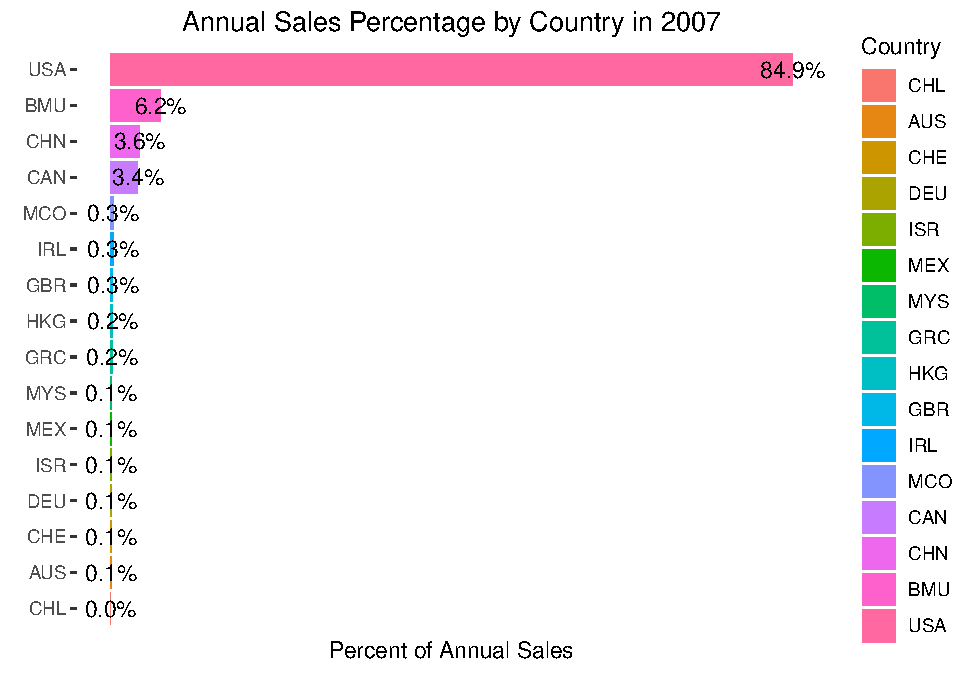
\includegraphics{Main_files/figure-latex/unnamed-chunk-19-1.pdf}


\end{document}
